
\appendix % začátek příloh

% hacks to remove the header and move page numbers into the margin

\pagestyle{appendix}
\newgeometry{textheight=760pt}

% ok so this is ugly as sin, but \leftmark and \rightmark didn't work with 
%  the phantom sections, so we redefine leftmark manually and use it on both sides

\renewcommand{\leftmark}{Appendix A.1: GEX Hub Schematics, Revision 1}
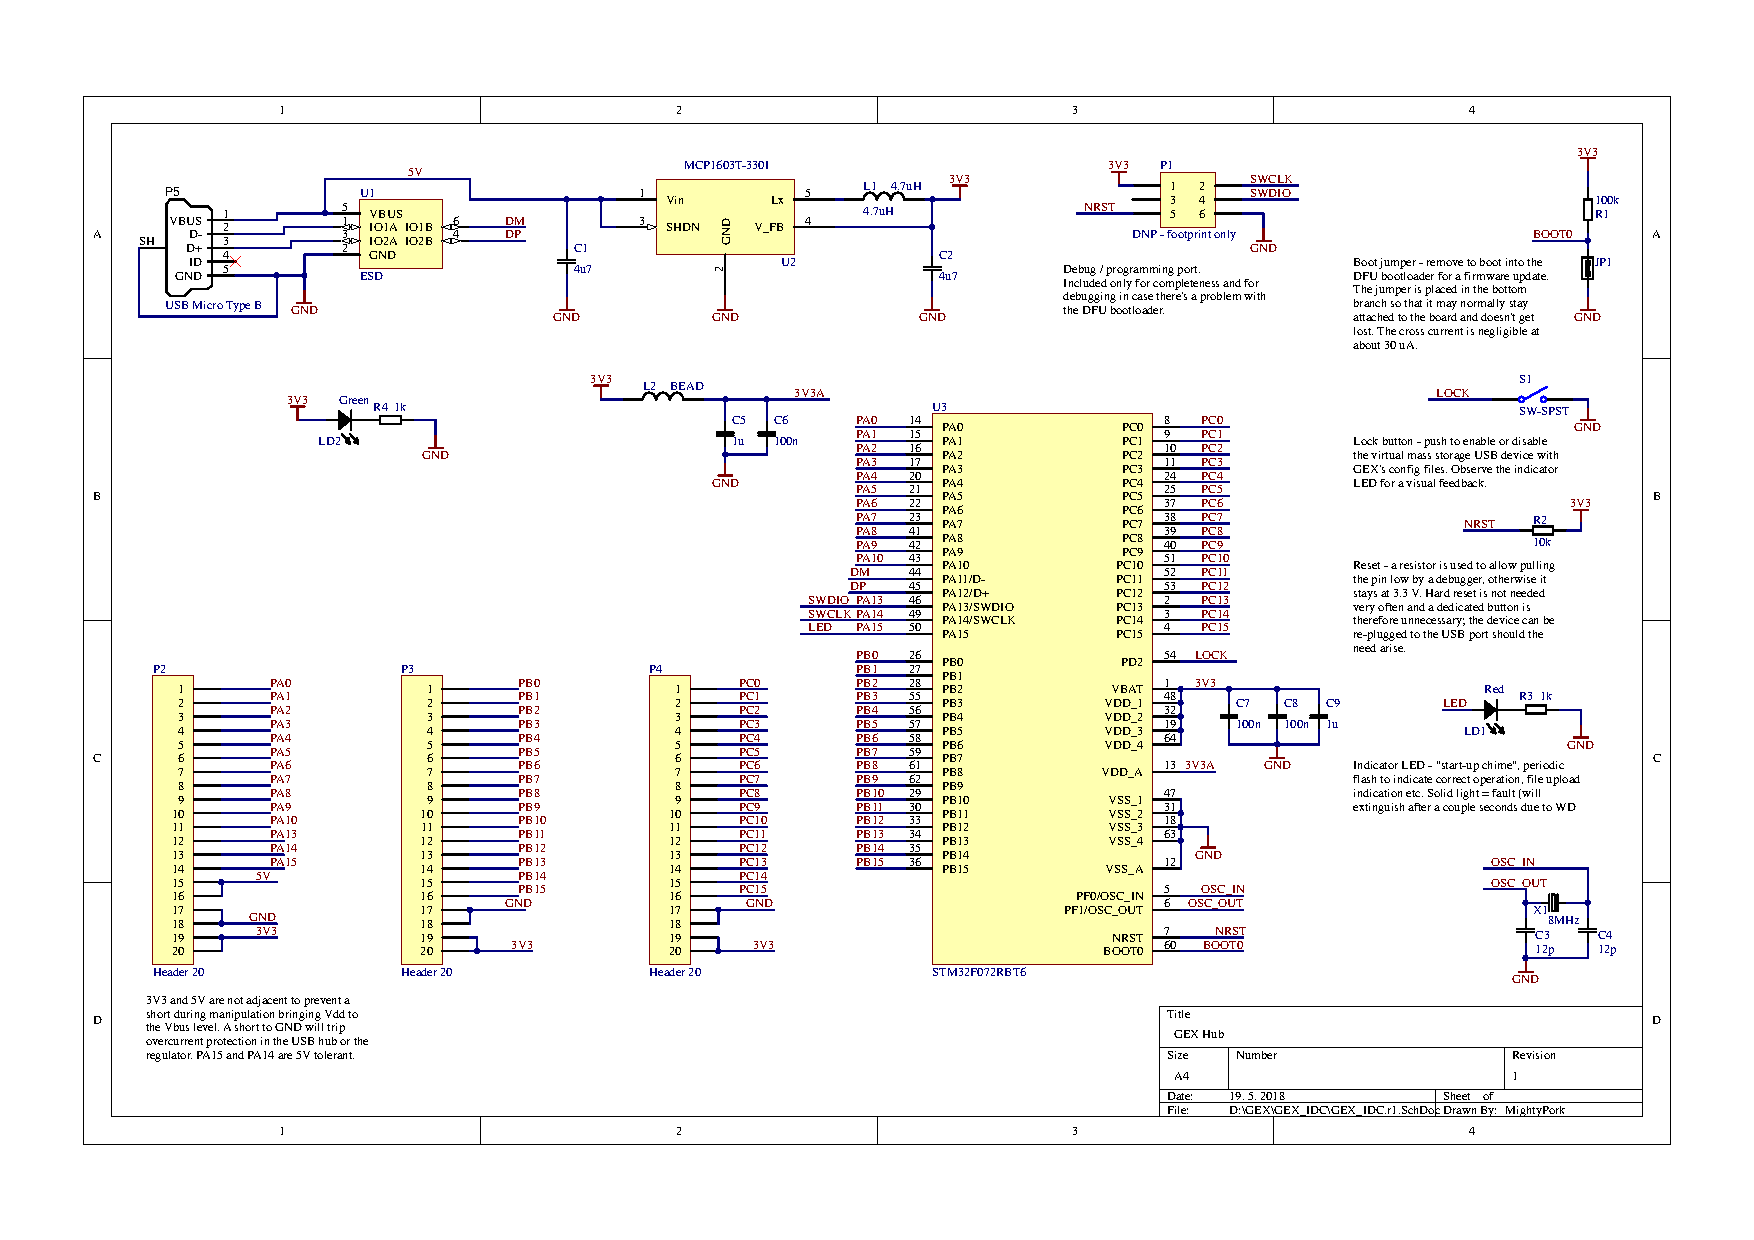
\includepdf[angle=90,pagecommand={%
	\phantomsection\addcontentsline{toc}{chapter}{A{\enspace}GEX Hub Schematics}%
	\label{apx:gex_hub}%
	\phantomsection\addcontentsline{toc}{section}{A.1 GEX Hub Revision 1}%
	\label{apx:gex_hub1}%
}]{schema/GexHubSchemRev1.pdf}

\renewcommand{\leftmark}{Appendix A.2: GEX Hub Schematics, Revision 2}
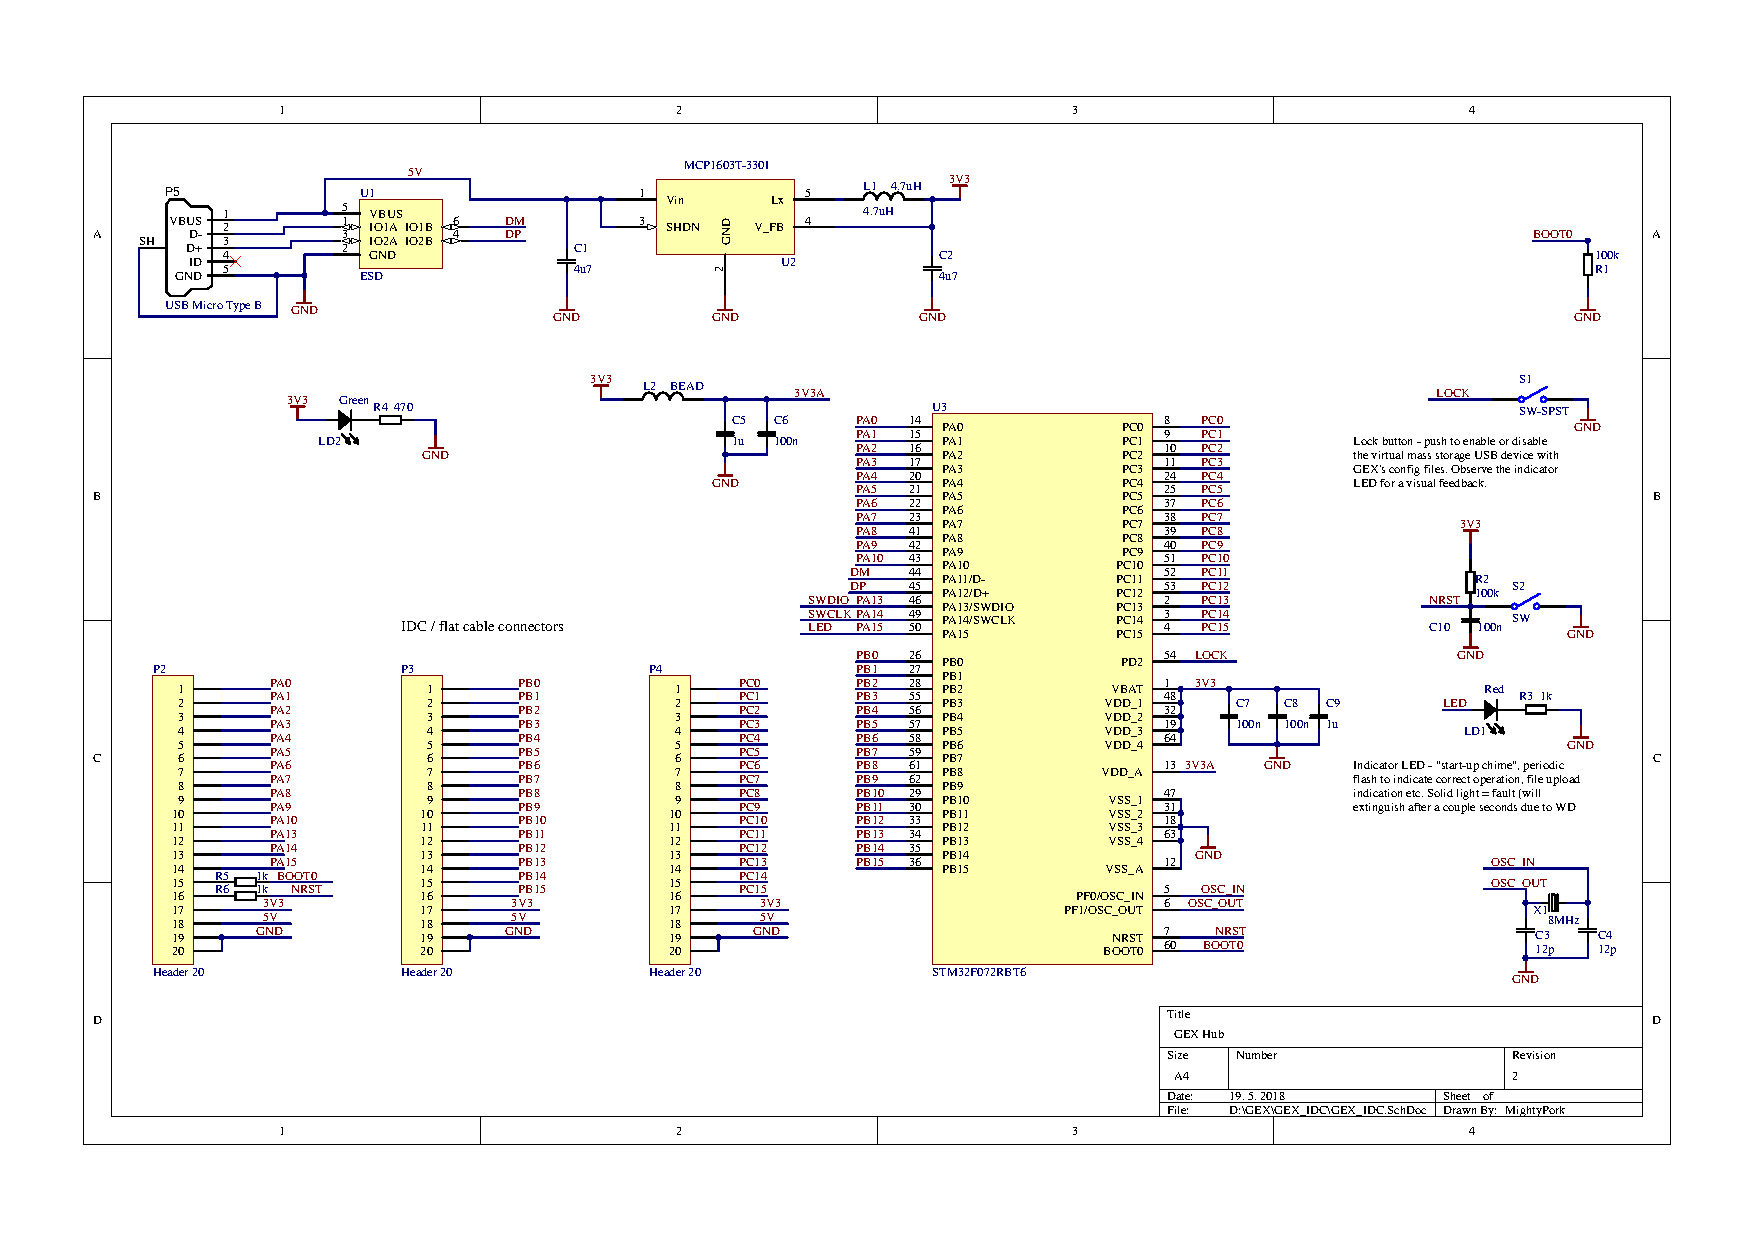
\includepdf[angle=90,pagecommand={%
	\phantomsection\addcontentsline{toc}{section}{A.2 GEX Hub Revision 2}%
	\label{apx:gex_hub2}%
}]{schema/GexHubSchemRev2.pdf}


\renewcommand{\leftmark}{Appendix B.1: GEX Zero Schematics, Revision 1}
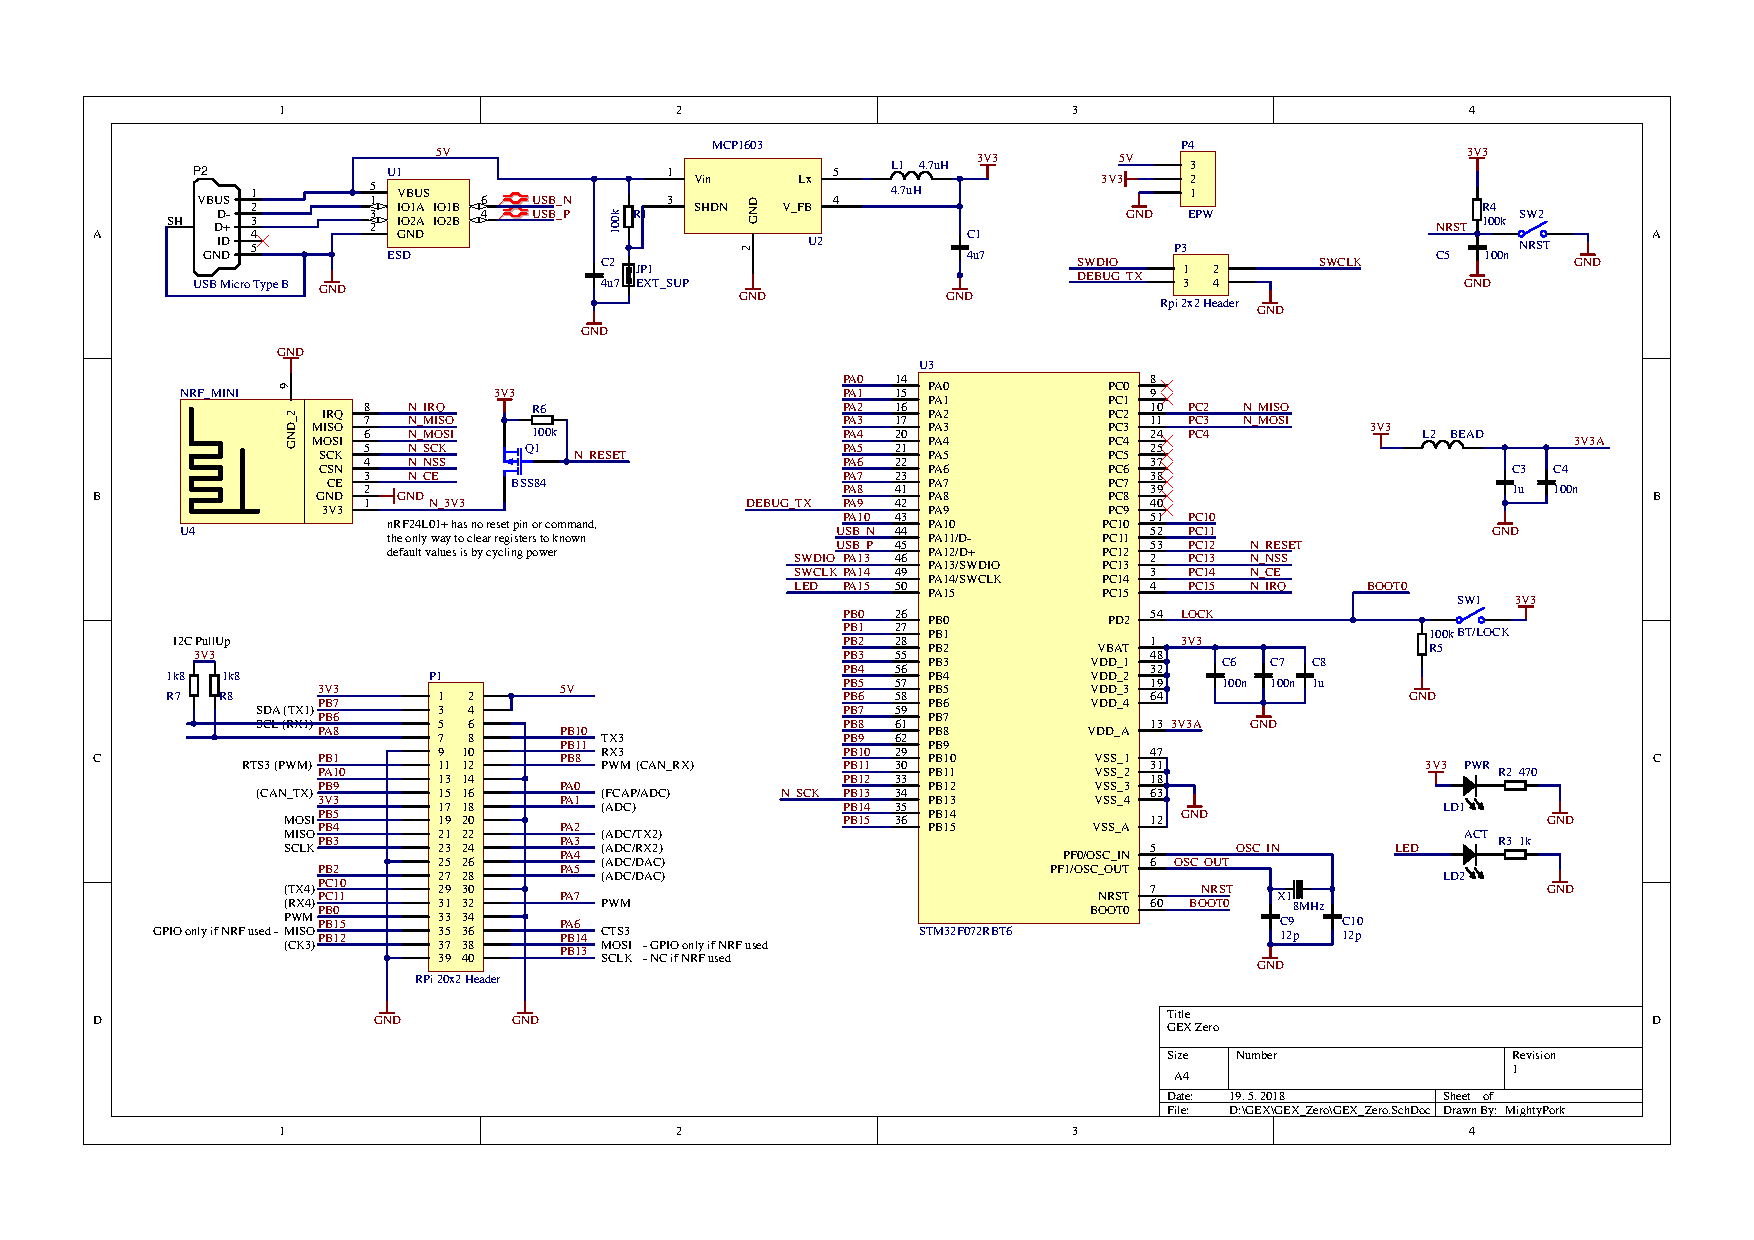
\includepdf[angle=90,pagecommand={%
	\phantomsection\addcontentsline{toc}{chapter}{B{\enspace}GEX Zero Schematics}%
	\label{apx:gex_zero}%
	\phantomsection\addcontentsline{toc}{section}{B.1 GEX Zero Revision 1}%
	\label{apx:gex_zero1}%
}]{schema/GexZeroSchemRev1.pdf}

\renewcommand{\leftmark}{Appendix B.2: GEX Zero Schematics, Revision 2}
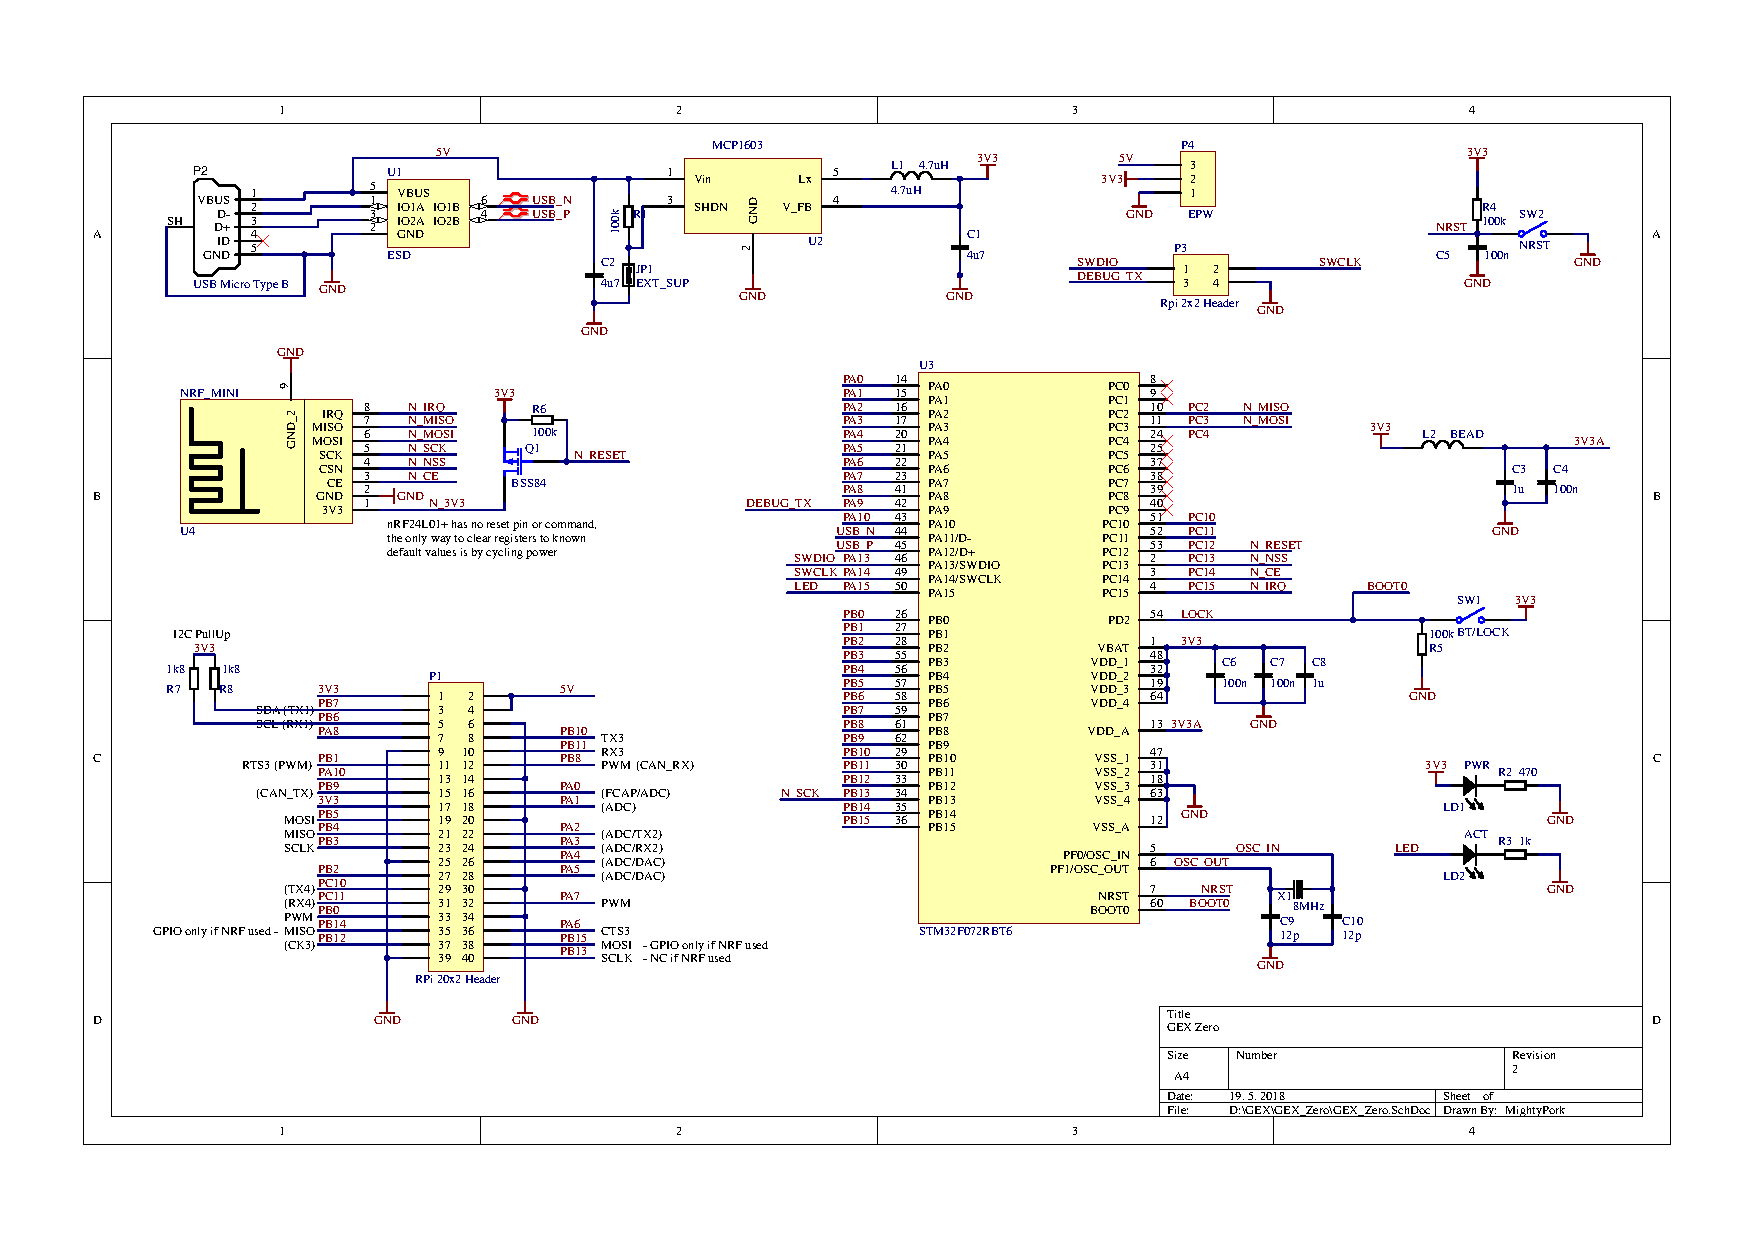
\includepdf[angle=90,pagecommand={%
	\phantomsection\addcontentsline{toc}{section}{B.2 GEX Zero Revision 2}%
	\label{apx:gex_zero2}%
}]{schema/GexZeroSchemRev2.pdf}


\renewcommand{\leftmark}{Appendix C: Wireless Gateway Schematics}
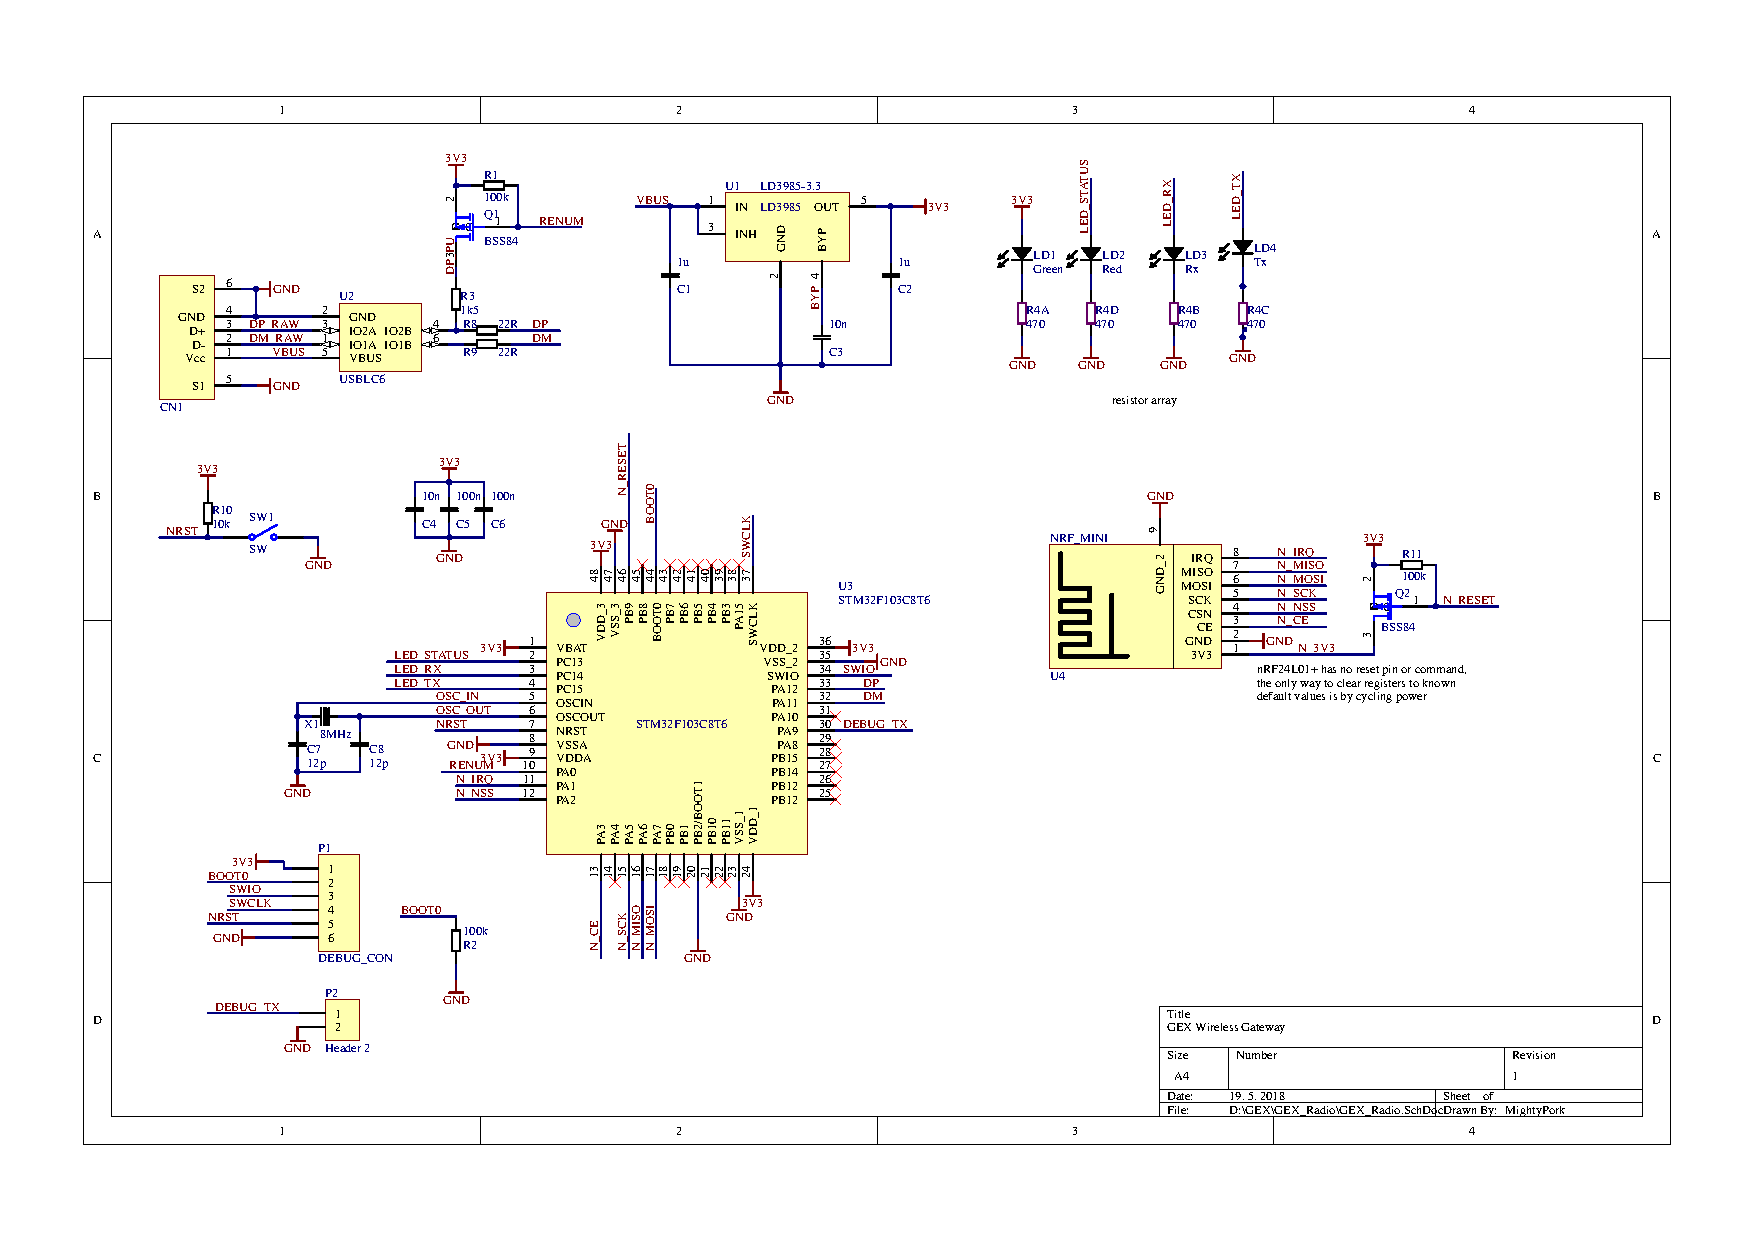
\includepdf[angle=90,pagecommand={%
	\phantomsection\addcontentsline{toc}{chapter}{C{\enspace}Wireless Gateway Schematics}%
	\label{apx:gex_wgw}%
}]{schema/GexRadioSchemRev1.pdf}

\newgeometry{textheight=665pt}
\setcounter{chapter}{3}
\renewcommand{\leftmark}{}
{\let\clearpage\relax \chapter{Content of the Attached CD}}

The attached CD (or archive, when downloaded in electronic form) contains source code of the embedded firmware, the client libraries, hardware projects, schematics, and material relating to the paper itself.

\begin{minipage}[t]{.45\textwidth}

\begin{Verbatim}
 ├── Firmware
 ├── Hardware
 │   ├── GEX HUB
 │   ├── GEX Zero
 │   ├── GEX Radio Dongle
 │   └── Zero+Hub+Dongle panel
 ├── Software
 │   ├── gex_client_c
 │   └── gex_client_py
 ├── Photos
 └── Thesis
     ├── Diagrams
     ├── References
     ├── Source
     └── GEX_Thesis.pdf
\end{Verbatim}
\end{minipage}
\begin{minipage}[t]{.55\textwidth}
\textbf{Firmware source code and binaries} \\
\textbf{Hardware projects, schematics, gerbers} \\
\null{\quad}GEX Hub\\
\null{\quad}GEX Zero\\
\null{\quad}Wireless gateway\\
\null{\quad}Panelized gerbers for manufacturing\\
\textbf{Documentation photos} \\
\textbf{Client libraries} \\
\null{\quad}C library\\
\null{\quad}Python library\\
\textbf{Thesis materials} \\
\null{\quad}Draw.io diagram data \\
\null{\quad}Referenced papers and documents \\
\null{\quad}\LaTeX\xspace source code, figures \\
\null{\quad}Electronic form of the thesis
\end{minipage}

\section*{Updates On-line}
Please note that the project is open-source and will continue to be developed and expanded after the submission of the paper. The attached source code and firmware images may not be up-to-date with the latest corrections and improvements.


\noindent
The full electronic text, the attachments disk image, and the latest source code may be obtained at the following URLs:

\begin{itemize}
\item Thesis download page \dots \url{https://www.ondrovo.com/cvut/dp/}
\item Source code repositories \dots \url{https://github.com/gexpander}
\item Project page \dots \url{https://gexpander.github.io/}
\end{itemize}

